\documentclass[11pt]{article}
\usepackage{../../Utility/Template}
\usepackage[raggedright]{titlesec}
\setcounter{secnumdepth}{5}
\setcounter{tocdepth}{5}
\usepackage{hyperref}
\usepackage{listings}
\usepackage{pdflscape}
\usepackage{enumitem}
\usepackage{afterpage}
\usepackage{float}

\setlength{\abovecaptionskip}{0pt plus 3pt minus 2pt}

\titleformat{\paragraph}[hang]{\normalfont\normalsize\bfseries}{\theparagraph}{1em}{}
\titlespacing*{\paragraph}{0pt}{3.25ex plus 1ex minus .2ex}{0.5em}
 
\definecolor{coloreRossoChiaro}{HTML}{934037}

\begin{document}
\newcommand{\Titolo}{\Glossario}

\newcommand{\Redattori}{\SP{} \newline	\ZM{} \newline \RA{} \newline \SH{}}

\newcommand{\Verificatori}{\BM{} \newline \PA{}}

\newcommand{\Approvatore}{\SG{}}

\newcommand{\Distribuzione}{\Proponente{} \newline \VT{} \newline \CR{} \newline Gruppo \Gruppo{}}

\newcommand{\Uso}{Esterno}

\newcommand{\DescrizioneDoc}{Il glossario serve per dare una definizione e chiarire il significato di alcuni termini presenti nella documentazione fornita.}

\newcommand{\pathimg}{../../Utility/images/logo2.png}

\newcommand{\Versionedoc}{1.0.0}
% info generali 

\newcommand{\NomeProgetto}{\textit{HD Viz}}

% fornitore
\newcommand{\Gruppo}{\textit{CodeBusters}}
\newcommand{\Mail}{codebusterswe@gmail.com}

% committenti
\newcommand{\Committente}{\VT \newline \CR}
\newcommand{\VT}{Prof. Vardanega Tullio}
\newcommand{\CR}{Prof. Cardin Riccardo}

% proponenti
\newcommand{\Proponente}{\textit{Zucchetti}}

% codebusters
\newcommand{\SG}{Sassaro Giacomo}
\newcommand{\BM}{Baldisseri Michele}
\newcommand{\ZM}{Zenere Marco}
\newcommand{\PA}{Pirolo Alessandro}
\newcommand{\SP}{Scialpi Paolo}
\newcommand{\SH}{Safdari Hossain}
\newcommand{\RA}{Rago Alessandro}

% ruoli
\newcommand{\Responsabile}{Responsabile di Progetto}
\newcommand{\Amministratore}{Amministratore di Progetto}

% documenti

\newcommand{\SdF}{\textit{Studio di Fattibilità}}
\newcommand{\SdFv}[1]{\textit{Studio di Fattibilità {#1}}}
\newcommand{\PdQ}{\textit{Piano di Qualifica}}
\newcommand{\PdQv}[1]{\textit{Piano di Qualifica {#1}}}
\newcommand{\PdP}{\textit{Piano di Progetto}}
\newcommand{\PdPv}[1]{\textit{Piano di Progetto {#1}}}
\newcommand{\NdP}{\textit{Norme di Progetto}}
\newcommand{\NdPv}[1]{\textit{Norme di Progetto {#1}}}
\newcommand{\AdR}{\textit{Analisi dei Requisiti}}
\newcommand{\AdRv}[1]{\textit{Analisi dei Requisiti {#1}}}
\newcommand{\Glossario}{\textit{Glossario}}
\newcommand{\Glossariov}[1]{\textit{Glossario {#1}}}
\newcommand{\MM}{\textit{Manuale Manutentore}}
\newcommand{\MMv}[1]{\textit{Manuale Manutentore {#1}}}
\newcommand{\MU}{\textit{Manuale Utente}}
\newcommand{\MUv}[1]{\textit{Manuale Utente {#1}}}

% comandi generali
\newcommand{\glo}[1]{#1\ap{G}}
%\newcommand{\glo}[1]{\textsc{#1\textsuperscript{\textit{G}}}}

\setlength{\parindent}{-0.1em}
\frontespizio 
\fancydoc
\newpage	
\section*{Registro delle modifiche}
{
\rowcolors{2}{colorePanna}{coloreGrigietto}
\renewcommand{\arraystretch}{1.5}
\centering
\begin{longtable}{c C{2.6cm} C{3cm} C{3cm} C{5cm}}
\rowcolor{coloreRosso}
\textcolor{white}{\textbf{Versione}}&
\textcolor{white}{\textbf{Data}}&
\textcolor{white}{\textbf{Nominativo}}&
\textcolor{white}{\textbf{Ruolo}}&
\textcolor{white}{\textbf{Descrizione}}\\	
\endhead

1.0.0 & 08/01/2021 & \SG{} & Responsabile & Approvazione del documento \\

0.3.0 & 04/01/2021 & \SH{} & Verificatore & Revisione complessiva del documento \\

0.2.6 & 22/12/2020 & \BM{} & Responsabile & Stesura \S A e \S B \\

0.2.5 & 21/12/2020 & \BM{} & Responsabile & Stesura \S 6\\

0.2.4 & 21/12/2020 & \SG{} & Responsabile & Aggiunti grafici \\

0.2.3 & 21/12/2020 & \BM{} & Responsabile & Stesura \S 5.3 e \S 5.4\\

0.2.2 & 20/12/2020 & \SG{} & Responsabile & Fine stesura \S 5.2 e stesura \S 5.5 \\

0.2.1 & 20/12/2020 & \BM{} & Responsabile & Stesura \S 5.3 e \S 5.4\\

0.2.0 & 19/12/2020 & \ZM{} & Verificatore & Revisione complessiva del documento \\

0.1.6 & 19/12/2020 & \SG{} & Responsabile & Inizio stesura \S 5 \\

0.1.5 & 18/12/2020 & \PA{} & Amministratore & Fine stesura \S 4.3\\

0.1.4 & 18/12/2020 & \SG{} & Responsabile & Stesura \S 4.4 \\

0.1.3 & 17/12/2020 & \BM{} & Responsabile & Stesura \S 4.2 e iniziata \S 4.3 \\

0.1.2 & 17/12/2020 & \SG{} & Responsabile & Stesura \S 4.1 \\

0.1.1 & 17/12/2020 & \SG{},\newline \BM{} & Responsabili & Stesura \S 3.2 \\

0.1.0 & 17/12/2020 & \ZM{} & Verificatore & Revisione complessiva del documento \\

0.0.5 & 16/12/2020 & \BM{} & Responsabile & Stesura \S 2.2 e \S 2.3 \\
		
0.0.4 & 15/12/2020 & \PA{} & Amministratore & Inizio stesura \S 2 \\

0.0.3 & 15/12/2020 & \SG{} & Responsabile & Stesura \S 3.1 \\

0.0.2 & 14/12/2020 & \PA{} & Amministratore & Aggiunta \S 1 \\

0.0.1 & 14/12/2020 & \SG{} & Responsabile & Creata struttura del documento Latex \\
		
\end{longtable}
}

\newpage
\tableofcontents
\newpage
\listoftables
\newpage
\listoffigures
\newpage
\section{Introduzione}
\subsection{Scopo del documento}
Questo documento ha lo scopo di fornire tutte le informazioni relative al sistema di controllo di qualità per i processi ed i prodotti, basandosi su assunti misurabili ma adattati alle esigenze del proprio progetto.
Esso deve implementare degli standard che permettano il miglioramento continuo, tracciando periodicamente tramite misurazioni i risultati ottenuti sfruttandoli per definire azioni migliorative. All'interno del \textit{Piano di Qualifica} vengono anche raccolte le definizioni dei test, il loro stato e il loro tracciamento. 

\subsection{Scopo del capitolato}
Oggigiorno, anche i programmi più tradizionali gestiscono e memorizzano una grande mole di dati; di conseguenza servono software in grado di eseguire un'analisi e un'interpretazione delle informazioni.\\
Il \glo{capitolato} C4 ha come obiettivo quello di creare un'applicazione di visualizzazione di dati con numerose dimensioni in modo da renderle comprensibili all'occhio umano.  Lo scopo del prodotto sarà quello di fornire all'utente diversi tipi di visualizzazioni e di algoritmi per la riduzione dimensionale in modo che, attraverso un processo esplorativo, l'utilizzatore del prodotto possa studiare tali dati ed evidenziarne degli eventuali \glo{cluster}. 

\subsection{Glossario}
Per evitare ambiguità relative alle terminologie utilizzate, è stato compilato il \Glossariov{2.0.0}. In questo documento sono riportati tutti i termini importanti e con un significato particolare. Questi termini sono evidenziati da una 'G' ad apice.

\subsection{Riferimenti}
\subsubsection{Riferimenti normativi}
\begin{itemize}	
\item \textbf{\NdPv{v 2.0.0}};
	
\item \textbf{Capitolato d'appalto C4 - HD Viz: visualizzazione di dati multidimensionali}:\\
	\textcolor{blue}{\url{https://www.math.unipd.it/~tullio/IS-1/2020/Progetto/C4.pdf}}

\end{itemize}

\subsubsection{Riferimenti informativi}
\begin{itemize}
	\item \textbf{Software Engineering - Ian Sommerville - 10 th Edition}: \\
	Parte 4 - Software Management
	\begin{itemize}
	\item Capitolo 24 - Quality Management:
		\begin{itemize}
			\item Paragrafo 24.1 - Software Quality (da pag. 703 a 705);
			\item Paragrafo 24.3 - Reviews and inspection (da pag. 710 a 714);
			\item Paragrafo 24.5 - Software measurement (da pag. 717 a 725).
		\end{itemize}
	\end{itemize}
	
	\item \textbf{Slide T12 del corso Ingegneria del Software - Qualità di prodotto}:\\
	\textcolor{blue}{\url{https://www.math.unipd.it/~tullio/IS-1/2020/Dispense/L12.pdf}}
	\begin{itemize}
		\item Slide 8 - I 7 principi del Sistema Qualità;
		\item Slide 12,13 - Cosa significa qualità SW;
		\item Slide 17 - Il processo di valutazione.
	\end{itemize}
	
	\item \textbf{Slide T13 del corso Ingegneria del Software - Qualità di processo}:\\
	\textcolor{blue}{\url{https://www.math.unipd.it/~tullio/IS-1/2020/Dispense/L13.pdf}}
		\begin{itemize}
		\item Slide 3 - Modello concettuale di processo;
		\item Slide 11 - I 5 livelli di maturità;
		\item Slide 23 - Riepilogo: la ricerca della qualità.
	\end{itemize}
	
	\item \textbf{Slide T14 del corso Ingegneria del Software - Verifica e validazione}:\\
	\textcolor{blue}{\url{https://www.math.unipd.it/~tullio/IS-1/2020/Dispense/L14.pdf}}
	\begin{itemize}
		\item Slide 6 - Verifica e validazione nello sviluppo; 
		\item Slide 15 - Analisi dinamica: tipi di test.
	\end{itemize}
	
	\item \textbf{Indice di Gulpease}:\\
	\textcolor{blue}{\url{https://it.wikipedia.org/wiki/Indice_Gulpease}}
	
	\item \textbf{Averege Cyclomatic complexity}:\\
	\textcolor{blue}{\url{https://eslint.org/docs/rules/complexity}}
	
\end{itemize}
\newpage
\section{Tecnologie coinvolte}
\subsection{Linguaggi}
\subsubsection{Javascript}
JavaScript è un linguaggio di programmazione  comunemente utilizzato nella programmazione Web per la creazione di effetti dinamici interattivi tramite funzioni di script invocati da eventi innescati a loro volta in vari modi dall'utente sulla pagina web in uso (mouse, tastiera, caricamento della pagina, ecc...).
\subsubsection{HTML5}
HTML5 è un linguaggio di markup per la strutturazione di pagine web. Viene utilizzato
nel progetto \NomeProgetto{} assieme a React per definire il frontend.
\subsubsection{CSS3}
Il CSS è un linguaggio usato per definire la formattazione di documenti HTML5, XHTML e XML, come ad esempio siti web e le relative pagine web.
Essendo il progetto \NomeProgetto{} composto di elementi HTML viene utilizzato il CSS per la loro stilizzazione. L’uso del CSS all'interno del progetto permette la separazione dei contenuti delle pagine HTML dal loro layout e permette una programmazione più chiara e facile da utilizzare, sia per gli autori delle pagine stesse sia per gli utenti, garantendo contemporaneamente anche il riutilizzo di codice ed una sua più facile manutenzione.

\subsection{Strumenti}
\subsubsection{PostgreSQL}
PostgreSQL è un completo \glo{DBMS} ad oggetti ed offre caratteristiche uniche nel suo genere che lo pongono per alcuni aspetti all'avanguardia nel settore delle basi di dati. Viene utilizzato nel progetto per il caricamento nell'applicazione di basi di dati prefatte a disposizione dell'utente.
\begin{itemize}
\item \textbf{Versione utilizzata:} 13.x .
\end{itemize}
\subsubsection{Npm}
Npm è un gestore di pacchetti per il linguaggio di programmazione JavaScript. È il gestore di pacchetti predefinito per l'ambiente di runtime JavaScript Node.js. Consiste in un client da linea di comando, chiamato anch'esso npm, e un database online di pacchetti pubblici e privati, chiamato npm registry.
Viene utilizzato dal gruppo per effettuare le operazioni di build del codice.
\begin{itemize}
\item \textbf{Versione utilizzata:} 7.x .
\end{itemize}
\subsubsection{ESLint}
ESLint è uno strumento di analisi del codice statico per identificare i modelli problematici trovati nel codice JavaScript. Le regole in ESLint sono configurabili e le regole personalizzate possono essere definite e caricate.
Nel progetto \NomeProgetto{} è stato utilizzato questo strumento principalmente per la segnalazione degli errori di sintassi, import che non vengono usati all'interno del progetto oppure variabili non utilizzate.
\begin{itemize}
\item \textbf{Versione utilizzata:} 7.15.0 .
\end{itemize}
\subsubsection{Babel}
Babel è un transcompiler JavaScript gratuito e open source che viene utilizzato principalmente per convertire il codice ECMAScript 2015+ in una versione compatibile con le versioni precedenti di JavaScript che può essere eseguita da motori JavaScript meno recenti.
\begin{itemize}
\item \textbf{Versione utilizzata:} 7.11.0 .
\end{itemize}

\subsection{Librerie e framework}
\subsubsection{D3.js}
D3.js è una libreria JavaScript per creare visualizzazioni dinamiche ed interattive partendo da dati organizzati, visibili attraverso un comune browser.
Questa libreria è stata utilizzata nel progetto \NomeProgetto{} per la creazione dei grafici per le rappresentazioni dei dati richiesti.
\begin{itemize}
\item \textbf{Versione utilizzata:} 6.x .
\end{itemize}
\subsubsection{React}
React è una libreria glo{JavaScript} per la creazione di interfacce utente utilizzato principalmente come base nello sviluppo di applicazioni a pagina singola o mobile.
Questa libreria è stata scelta per la realizzazione del progetto per poter facilitare lo sviluppo del frontend e avere più performance grazie al suo metodo di renderizzazione dei dati.
\begin{itemize}
\item \textbf{Versione utilizzata:} 17.0.1 .
\end{itemize}
\subsubsection{Node.js}
Node.js è un runtime system open source multipiattaforma orientato agli eventi per l'esecuzione di codice JavaScript, costruita sul motore JavaScript V8 di Google Chrome.
Node.js è stato utilizzato per lo sviluppo del progetto \NomeProgetto{} come strumento per l'utilizzio di Javascript lato server.
\begin{itemize}
\item \textbf{Versione utilizzata:} 14.16.0 .
\end{itemize}
\subsubsection{React Bootstrap}
Bootstrap è un framework che permette la creazione di siti e applicazioni per il Web responsive. Questa libreria chiamata React Bootstrap permette di costruire componenti come se fossero componenti React veri e propri senza dipendenze non necessarie. Essa è stata utilizzata per il progetto perchè contiene modelli di progettazione basati su HTML e CSS, sia per la tipografia, che per le varie componenti dell'interfaccia, come modal, pulsanti, burger menù e form.
\begin{itemize}
\item \textbf{Versione utilizzata:} 1.5.2 .
\end{itemize}
\subsubsection{MobX}
MobX è una libreria appositamente creata per React che permette la gestione dello \glo{state} dei componenti in maniera semplice e scalabile. Nel progetto \NomeProgetto{} è stata utilizza questa libreria per l'implementazione del design pattern Observer.
\begin{itemize}
\item \textbf{Versione utilizzata:} 6.1.x .
\end{itemize}
\subsubsection{Druid.js}
DruidJS è una libreria JavaScript per la riduzione della dimensionalità. Con la riduzione della dimesionalità è possibile proiettare dati ad alta dimensionalità su una dimensionalità inferiore mantenendo le proprietà dei dati specifiche del metodo. DruidJS semplifica la proiezione di un set di dati con i metodi di riduzione della dimensionalità implementati.
Nel progetto \NomeProgetto questa libreria viene usata per implementare il processo di riduzione dimensionale.
\begin{itemize}
\item \textbf{Versione utilizzata:} 0.3.5 .
\end{itemize}
\subsubsection{Express}
Express è un framework open source per applicazioni web per Node.js. È stato progettato per creare web application e API ed è ormai definito il server framework standard de facto per Node.js.
Nel progetto \NomeProgetto Express fa da intermediario tra web app e database, agevolando il collegamento.
\begin{itemize}
\item \textbf{Versione utilizzata:} 4.17.1 .
\end{itemize}
\subsubsection{Jest} 
Jest è un framework di test JavaScript open-source gestito da Facebook. Funziona con progetti che utilizzano Babel, TypeScript, Node.js, React, Angular, Vue.js e Svelte.
\begin{itemize}
\item \textbf{Versione utilizzata:} 26.x .
\end{itemize}
\subsubsection{React Testing Library}
La libreria React Testing Library è una soluzione per testare i componenti React; viene utilizzata nel progetto \NomeProgetto{} per la stesura dei test.
\begin{itemize}
\item \textbf{Versione utilizzata:} 11.2.x .
\end{itemize}

\section{Configurazione}
In questa sezione vengono trattati in primo luogo i requisiti minimi necessari per l'utilizzo dell'applicazione \textit{HDViz} e successivamente come poter installare il prodotto in locale direttamente dal repository pubblico in GitHub.  
\subsection{Requisiti di sistema}
Per far si che le operazioni di installazione e avvio del prodotto avvengano correttamente e che si possa aver accesso a tutte le funzionalità, è necessario avere nella propria macchina i seguenti software.
{
\setlength\arrayrulewidth{0.95pt}
\renewcommand{\arraystretch}{1.5}
\begin{longtable}{C{3cm} C{3cm} C{9cm}}
\rowcolor{coloreRosso}

\textcolor{white}{\textbf{Software}}&
\textcolor{white}{\textbf{Versione}}&
\textcolor{white}{\textbf{Riferimento per il downlaod}} \\
\endfirsthead
\rowcolor{white}\multicolumn{3}{C{15cm}}{\textit{Continua nella pagina successiva...}}\\
\endfoot
\rowcolor{white}\caption{Requisiti di sistema}
\endlastfoot
	
	\textbf{Node.js} &
	14.16.x &
	\textcolor{blue}{\url{https://nodejs.org/it/}} \\
 
	\textbf{Npm} & 
	7.x &
	Integrato nel download di Node.js \\
	
	\textbf{PostgreSQL} &
	13.x &
	\textcolor{blue}{\url{https://www.postgresql.org/download/}} \\
\end{longtable}	

}
\subsection{Requisiti hardware}
Come definito nell'analisi dei requisti, per avere delle prestazioni accettabili dell'applicazione è preferibile avere almeno i seguenti componenti hardware.
{
\setlength\arrayrulewidth{0.95pt}
\renewcommand{\arraystretch}{1.5}
\begin{longtable}{C{4cm} C{4cm}}
\rowcolor{coloreRosso}

\textcolor{white}{\textbf{Componente}}&
\textcolor{white}{\textbf{Requisito}} \\
\endfirsthead
\endfoot
\rowcolor{white}\caption{Requisiti hardware}
\endlastfoot
	
	\textbf{Processore} &
	 Quad-Core 3,2 GHz \\
 
	\textbf{RAM} & 
	8GB DDR4 \\

\end{longtable}	
}

La connessione internet ideale dovrebbe essere di almeno 80Mb/s in download per assicurare i seguenti tempi di risposta (in secondi) della web app. 
{
\setlength\arrayrulewidth{0.95pt}
\renewcommand{\arraystretch}{1.5}
\begin{longtable}{C{2cm} C{10cm}}
\rowcolor{coloreRosso}

\textcolor{white}{\textbf{Tempo}}&
\textcolor{white}{\textbf{Operazione}} \\
\endfirsthead
\endfoot
\rowcolor{white}\caption{Prestazioni ottimali}
\endlastfoot
	
	\textbf{2} &
	Caricamento di un dataset di 2Mb;  \\
 
	\textbf{7} & 
	Applicazione di un algoritmo  di riduzione dimensionale con 4 dimensioni e 500 punti in totale; \\
	
	\textbf{2} &
	Visualizzazione di un grafico con 500 punti.  \\	
	
\end{longtable}	
}

\subsection{Browser}
L'applicazione è stata testata e quindi resa compatibile con le ultime versioni dei browser maggiormente utilizzati al momento.
{
\setlength\arrayrulewidth{0.95pt}
\renewcommand{\arraystretch}{1.5}
\begin{longtable}{C{4cm} C{4cm}}
\rowcolor{coloreRosso}

\textcolor{white}{\textbf{Browser}}&
\textcolor{white}{\textbf{Versione}} \\
\endfirsthead
\endfoot
\rowcolor{white}\caption{Browser e versioni compatibili}
\endlastfoot
	
	\textbf{Chrome} &
	 87 \\
 
	\textbf{Edge} & 
	79\\
	
	\textbf{Mozilla Firefox} &
	 84 \\
 
	\textbf{Safari} & 
	13.1 \\
	
\end{longtable}	
}

\subsection{Installazione}
Per installare il prodotto in locale è necessario seguire i passi qui riportati.
\begin{enumerate}
	\item Scaricare il codice come file .zip direttamente dal repository di CodeBusters-HDViz:
		\begin{center}
			\textcolor{blue}{\url{https://github.com/CodeBusterswe/CodeBusters-HDviz}}
		\end{center}	
	Oppure, con Git installato in locale, è possibile clonare il repositoty con il comando:
		\begin{center}
			\textcolor{darkgray}{\textbf{git clone https://github.com/CodeBusterswe/CodeBusters-HDviz}}
		\end{center}
      
	\item Localizzare da terminale la cartella in cui si è stato estratto/clonato il prodotto:  
		\begin{center}
			\textcolor{darkgray}{\textbf{cd percorso\textbackslash HDViz}}
 		\end{center}	
	\item Entrare nella cartella "client":
		\begin{center}
			\textcolor{darkgray}{\textbf{cd client}}
 		\end{center}	     
	\item A questo punto è necessario installare tutti i "node\_ modules", ossia tutte le dipendenze dichiarate nel "package.json". Questo è possibile lanciando il comando:
		\begin{center}
			\textcolor{darkgray}{\textbf{npm install}}
 		\end{center}		
	Ci vorrà al massimo qualche minuto. 
	\item Terminata l'installazione è subito possibile avviare l'applicazione con il comando:
		\begin{center}
			\textcolor{darkgray}{\textbf{npm start}}
 		\end{center}
	Al termine dell'operazione dovrebbe aprirsi in automatico l'applicazione. In caso contrario aprire un browser e inserire l'indirizzo:
	\begin{center}
		\textbf{localhost:3000} .
	\end{center}		
\end{enumerate}
  			
\newpage
\section{Strumenti per l'analisi e l'integrazione del codice}

{
\setlength\arrayrulewidth{0.95pt}
\renewcommand{\arraystretch}{1.5}
\begin{longtable}{C{3cm} | C{2cm} | C{10cm}}
\rowcolor{coloreRosso}

\textcolor{white}{\textbf{Strumento}}&
\textcolor{white}{\textbf{Versione}}&
\textcolor{white}{\textbf{Descrizione}} \\
\endfirsthead
\rowcolor{white}\multicolumn{3}{C{15cm}}{\textit{Continua nella pagina successiva...}}\\
\endfoot
\rowcolor{white}\caption{Strumenti per l'analisi e l'integrazione del codice}
\endlastfoot
	
\rowcolor{coloreRossoChiaro}
\multicolumn{3}{|c|}{\textcolor{white}{\textbf{Analisi statica}}} \\

\textbf{ESLint} & 7.15.0 & 
	Strumento di analisi statica utilizzato per la segnalazione degli errori di sintassi, per avere regole  d'indentazione uguali in tutti i file e per notifiche altri problemi comuni. \\

\rowcolor{coloreRossoChiaro}
\multicolumn{3}{|c|}{\textcolor{white}{\textbf{Analisi dinamica}}} \\

\textbf{Jest} & 26.x & 
\glo{Framework} di test utilizzato per l'analisi dinamica del codice. \\

\textbf{React Testing Library} & 11.2.x & 
Libreria usata per testare lo stato interno delle componenti React. \\

\rowcolor{coloreRossoChiaro}
\multicolumn{3}{|c|}{\textcolor{white}{\textbf{Continuous Integration}}} \\

\textbf{GitHub Actions} & - & 
Strumento fornito da GitHub per l'implementazione della CI/CD all'interno del proprio repository. \\

\textbf{SonarCloud} & - & 
Piattaforma per il controllo continuo della qualità e manutenibilità del codice.\\

\textbf{CodeCov} & - & 
Piattaforma per il controllo del code coverage.\\

\end{longtable}
}
\newpage
\section{Architettura}
\newpage
\section{Server Side}
\NomeProgetto{} è una web application che non richiede un'ampia comunicazione con il lato server. Esso è infatti utilizzato solo per l'interrogazione del database PostgreSQL, per permettere all'utente di caricare i suoi dati contenuti nel database. \\
Per questo motivo è stato deciso di non adottare una specifica architettura lato server. \\
I file dedicati sono contenuti nella cartella \texttt{server}, così organizzati:
\begin{itemize}
	\item \texttt{test} è la sottocartella contenente il file \textbf{server.test.js} utile a controllare che la connessione con il server avvenga correttamente; 
	\item \texttt{config} è la sottocartella contenente i file per la configurazione del database. All'interno del file \textbf{default.js} è infatti possibile cambiare i dati di acceso al DB con le proprie credenziali (figura \ref{config})
	\item \texttt{api} è la sottocartella contenente il file \textbf{DataSet.js}. Al suo interno sono presenti le API create con Express.js per la comunicazione del lato client dell'applicazione con il server sviluppato con Node.js.
\end{itemize}

\begin{figure}[hb]
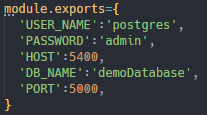
\includegraphics[width=8cm]{Images/credenziali}
\centering
\caption{Credenziali di default}
\label{config}
\end{figure}
\newpage
\section{Principali punti di estensione}


\clearpage
\documentclass[11pt]{article}
\usepackage{../../Utility/Template}
\usepackage{hyperref}
\usepackage{fancyhdr}
\usepackage{tocloft}
\renewcommand{\cftsecleader}{\cftdotfill{\cftdotsep}}

\begin{document}
\newcommand{\Titolo}{\Glossario}

\newcommand{\Redattori}{\SP{} \newline	\ZM{} \newline \RA{} \newline \SH{}}

\newcommand{\Verificatori}{\BM{} \newline \PA{}}

\newcommand{\Approvatore}{\SG{}}

\newcommand{\Distribuzione}{\Proponente{} \newline \VT{} \newline \CR{} \newline Gruppo \Gruppo{}}

\newcommand{\Uso}{Esterno}

\newcommand{\DescrizioneDoc}{Il glossario serve per dare una definizione e chiarire il significato di alcuni termini presenti nella documentazione fornita.}

\newcommand{\pathimg}{../../Utility/images/logo2.png}

\newcommand{\Versionedoc}{1.0.0}
% info generali 

\newcommand{\NomeProgetto}{\textit{HD Viz}}

% fornitore
\newcommand{\Gruppo}{\textit{CodeBusters}}
\newcommand{\Mail}{codebusterswe@gmail.com}

% committenti
\newcommand{\Committente}{\VT \newline \CR}
\newcommand{\VT}{Prof. Vardanega Tullio}
\newcommand{\CR}{Prof. Cardin Riccardo}

% proponenti
\newcommand{\Proponente}{\textit{Zucchetti}}

% codebusters
\newcommand{\SG}{Sassaro Giacomo}
\newcommand{\BM}{Baldisseri Michele}
\newcommand{\ZM}{Zenere Marco}
\newcommand{\PA}{Pirolo Alessandro}
\newcommand{\SP}{Scialpi Paolo}
\newcommand{\SH}{Safdari Hossain}
\newcommand{\RA}{Rago Alessandro}

% ruoli
\newcommand{\Responsabile}{Responsabile di Progetto}
\newcommand{\Amministratore}{Amministratore di Progetto}

% documenti

\newcommand{\SdF}{\textit{Studio di Fattibilità}}
\newcommand{\SdFv}[1]{\textit{Studio di Fattibilità {#1}}}
\newcommand{\PdQ}{\textit{Piano di Qualifica}}
\newcommand{\PdQv}[1]{\textit{Piano di Qualifica {#1}}}
\newcommand{\PdP}{\textit{Piano di Progetto}}
\newcommand{\PdPv}[1]{\textit{Piano di Progetto {#1}}}
\newcommand{\NdP}{\textit{Norme di Progetto}}
\newcommand{\NdPv}[1]{\textit{Norme di Progetto {#1}}}
\newcommand{\AdR}{\textit{Analisi dei Requisiti}}
\newcommand{\AdRv}[1]{\textit{Analisi dei Requisiti {#1}}}
\newcommand{\Glossario}{\textit{Glossario}}
\newcommand{\Glossariov}[1]{\textit{Glossario {#1}}}
\newcommand{\MM}{\textit{Manuale Manutentore}}
\newcommand{\MMv}[1]{\textit{Manuale Manutentore {#1}}}
\newcommand{\MU}{\textit{Manuale Utente}}
\newcommand{\MUv}[1]{\textit{Manuale Utente {#1}}}

% comandi generali
\newcommand{\glo}[1]{#1\ap{G}}
%\newcommand{\glo}[1]{\textsc{#1\textsuperscript{\textit{G}}}}

\setlength{\parindent}{-0.1em}
\frontespizio
\fancydoc
\newpage	
\section*{Registro delle modifiche}
{
\rowcolors{2}{colorePanna}{coloreGrigietto}
\renewcommand{\arraystretch}{1.5}
\centering
\begin{longtable}{c C{2.6cm} C{3cm} C{3cm} C{5cm}}
\rowcolor{coloreRosso}
\textcolor{white}{\textbf{Versione}}&
\textcolor{white}{\textbf{Data}}&
\textcolor{white}{\textbf{Nominativo}}&
\textcolor{white}{\textbf{Ruolo}}&
\textcolor{white}{\textbf{Descrizione}}\\	
\endhead

1.0.0 & 08/01/2021 & \SG{} & Responsabile & Approvazione del documento \\

0.3.0 & 04/01/2021 & \SH{} & Verificatore & Revisione complessiva del documento \\

0.2.6 & 22/12/2020 & \BM{} & Responsabile & Stesura \S A e \S B \\

0.2.5 & 21/12/2020 & \BM{} & Responsabile & Stesura \S 6\\

0.2.4 & 21/12/2020 & \SG{} & Responsabile & Aggiunti grafici \\

0.2.3 & 21/12/2020 & \BM{} & Responsabile & Stesura \S 5.3 e \S 5.4\\

0.2.2 & 20/12/2020 & \SG{} & Responsabile & Fine stesura \S 5.2 e stesura \S 5.5 \\

0.2.1 & 20/12/2020 & \BM{} & Responsabile & Stesura \S 5.3 e \S 5.4\\

0.2.0 & 19/12/2020 & \ZM{} & Verificatore & Revisione complessiva del documento \\

0.1.6 & 19/12/2020 & \SG{} & Responsabile & Inizio stesura \S 5 \\

0.1.5 & 18/12/2020 & \PA{} & Amministratore & Fine stesura \S 4.3\\

0.1.4 & 18/12/2020 & \SG{} & Responsabile & Stesura \S 4.4 \\

0.1.3 & 17/12/2020 & \BM{} & Responsabile & Stesura \S 4.2 e iniziata \S 4.3 \\

0.1.2 & 17/12/2020 & \SG{} & Responsabile & Stesura \S 4.1 \\

0.1.1 & 17/12/2020 & \SG{},\newline \BM{} & Responsabili & Stesura \S 3.2 \\

0.1.0 & 17/12/2020 & \ZM{} & Verificatore & Revisione complessiva del documento \\

0.0.5 & 16/12/2020 & \BM{} & Responsabile & Stesura \S 2.2 e \S 2.3 \\
		
0.0.4 & 15/12/2020 & \PA{} & Amministratore & Inizio stesura \S 2 \\

0.0.3 & 15/12/2020 & \SG{} & Responsabile & Stesura \S 3.1 \\

0.0.2 & 14/12/2020 & \PA{} & Amministratore & Aggiunta \S 1 \\

0.0.1 & 14/12/2020 & \SG{} & Responsabile & Creata struttura del documento Latex \\
		
\end{longtable}
}

\newpage
\tableofcontents
\newpage
\section*{A}
\markright{}
\addcontentsline{toc}{section}{A}

\subsection*{Android}
Sistema operativo per dispositivi mobili sviluppato da Google. È un software \glo{open source} con controparti proprietarie che, dal 2017, risulta essere il sistema operativo mobile più diffuso al mondo. 
 
\subsection*{Angular}
\glo{Framework} \glo{open source} per lo sviluppo di applicazioni web eseguite interamente dal web browser dopo essere state scaricate dal web server.

\subsection*{API}
Acronimo di Application Programming Interface. Si indica un  insieme  di  procedure disponibili al programmatore, di solito  raggruppate a formare un set di strumenti specifici per lo svolgimento di un determinato compito all'interno di un certo programma. Talvolta le API sono offerte tramite servizi a pagamento, oppure potrebbero essere funzionalità gratuite, come librerie software disponibili in un certo linguaggio di programmazione.

\subsection*{AWS}
Acronimo di Amazon Web Service. Azienda di proprietà di Amazon che offre diversi servizi di cloud computing su una piattaforma online.

\subsection*{AWS API Gateway}
Servizio \glo{AWS} per la creazione, pubblicazione, gestione e monitoraggio di \glo{API} che accedono ad altri servizi AWS o utilizzano dati archiviati in un AWS Cloud.

\subsection*{AWS Appsync}
Servizio \glo{AWS} utile per velocizzare la creazione di API gestendo attività che prevedono l'utilizzo di un \glo{AWS Dynamo DB} o un \glo{AWS Lambda}.

\subsection*{AWS Cognito Identity}
Servizio \glo{AWS} che permette di aggiungere velocemente diversi metodi di registrazione nell'\glo{API}. Permette quindi all'utente di registrarsi utilizzando un profilo che già possiede di un altro social network, come per esempio Amazon, Facebook o Google. 

\subsection*{AWS Dynamo DB}
\glo{Database} \glo{NoSQL} di \glo{AWS} completamente gestito che permette agli sviluppatori di caricare un qualsiasi volume di dati per la propria applicazione. DynamoDB permette prestazioni elevate e tempi di latenza bassi per eseguire applicazioni web che altrimenti sovraccaricherebbero i database relazionali tradizionali.

\subsection*{AWS Gamelift}
Servizio \glo{AWS} che si occupa di distribuire, gestire e dimensionare i server cloud utilizzati per giochi multigiocatore. Migliora la latenza per i giocatori connessi ottimizzando i costi.

\subsection*{AWS Lambda}
Servizio \glo{AWS} che permette di gestire codice scritto senza dover occuparsi dell'amministrazione di esso o della gestione dei server. Lambda si occupa anche di calibrare costantemente le risorse necessarie, favorendo efficienza nel loro utilizzo. 

\subsection*{AWS S3}
Servizio \glo{AWS} di storage di oggetti che offre scalabilità, sicurezza e alte prestazioni sui dati che vengono salvati al suo interno. Permette di gestire ed organizzare con facilità una qualsiasi quantità di dati, nella massima sicurezza e per una vasta gamma di casi d'uso.

\newpage
\section*{B}
\markright{}
\addcontentsline{toc}{section}{B}
\subsection*{Ad esempio:}
Modo di dare una definizione, copiare subsection*{} e inserire tra le parentesi graffe la parola da definire. La definizione deve essere apposta sotto.
\newpage
\section*{C}
\markright{}
\addcontentsline{toc}{section}{C}

\subsection*{Capitolato}
Documento redatto dal cliente in cui vengono specificati i vincoli contrattuali (prezzo e scadenze) per lo sviluppo di un determinato prodotto software. Tale documento viene presentato in un bando d’appalto e serve a trovare qualcuno che possa svolgere il lavoro richiesto.

\subsection*{Cloud}
Vasta rete di server remoti ubicati in tutto il mondo, collegati tra loro e che operano come un unico ecosistema. Questi server possono archiviare e gestire dati, eseguire applicazioni o distribuire contenuti o servizi. L'accesso avviene online, da qualsiasi dispositivo con connessione Internet.

\subsection*{CloudFormation}
Strumento di \glo{AWS} che permette di modellare una raccolta di risorse AWS e gestirle nell'intero arco di ciclo di vita del prodotto.

\subsection*{Cluster}
Un cluster è un insieme di oggetti che presentano tra loro delle similarità e, allo stesso modo, delle dissimilarità con oggetti in altri cluster.

\subsection*{Code folding}
È una caratteristica di alcuni editor di testo e ambienti di sviluppo. Permette di nascondere delle porzioni di un file di codice mentre si lavora ad altre parti dello stesso file. Ciò permette agli sviluppatori di gestire più comodamente file molto lunghi all'interno di un'unica finestra.

\subsection*{CSS}
Acronimo di Cascading Style Sheets. Linguaggio usato per definire la formattazione di documenti HTML, XHTML e XML, ad esempio i siti web e relative pagine web.

\subsection*{CSV}
Acronimo di comma-separated values. Formato di file basato su file di testo utilizzato per l'importazione ed esportazione (ad esempio da fogli elettronici o database) di una tabella di dati. 


\subsection*{Compiti}
Attività assegnate ai membri del gruppo; devono essere svolte entro un determinato tempo.
\newpage
\section*{D}
\markright{}
\addcontentsline{toc}{section}{D}

\subsection*{Database}
Letteralmente "base di dati". Rappresenta la versione digitale di un archivio di informazioni, ossia memorizza e organizza grandi moli di dati all'interno di dischi rigidi.

\subsection*{D3.js}
È una libreria \glo{JavaScript} per creare visualizzazioni dinamiche ed interattive partendo da dati organizzati, visibili attraverso un comune browser.

\subsection*{Deep learning}
Insieme di tecniche basate su reti neurali artificiali organizzate in diversi strati, dove ogni strato calcola i valori per quello successivo affinché l'informazione venga elaborata in maniera sempre più completa.

\subsection*{Dendrogramma}
Nelle tecniche di clustering viene utilizzato per fornire una rappresentazione grafica del processo di raggruppamento delle istanze.

\subsection*{Design pattern}
Un design pattern descrive una soluzione generale a un problema di progettazione ricorrente, gli attribuisce un nome, astrae e identifica gli aspetti principali della struttura utilizzata per la soluzione del problema, identifica le classi e le istanze partecipanti e la distribuzione delle responsabilità, descrive quando e come può essere applicato. 

\subsection*{Discord}
Applicazione \glo{multipiattaforma} basta sulla tecnologia VoIP (Voice over Internet Protocol) che consente di creare gruppi di messaggistica e videoconferenze. Questa applicazione funziona sia sui dispositivi mobili sia su browser.

\subsection*{Docker}
Progetto open source che automatizza il rilascio di applicazioni all'utente all'interno di contenitori software.



\newpage
\section*{E}
\markright{}
\addcontentsline{toc}{section}{E}

\subsection*{E-Commerce}
Insieme delle transazioni per la commercializzazione di beni e servizi tra produttore e consumatore realizzate tramite Internet.

\subsection*{Epsilon}
Nell'algoritmo \glo{t-SNE} per Epsilon si intende il tasso di apprendimento. Questo parametro controlla la frequenza di aggiornamento del gradiente.

\subsection*{Express.js}
È un \glo{framework} \glo{open source} per applicazioni web per Node.js sotto Licenza MIT. È stato progettato per creare web application e API, ed è ormai definito il server framework standard per Node.js.

\subsubsection*{EsLint} 
È uno strumento di analisi statica del codice statica che permette di individuare gli errori e scrivere un programma corretto in \glo{Javascript}.   
\newpage
\section*{F}
\markright{}
\addcontentsline{toc}{section}{F}
\subsection*{Ad esempio:}
Modo di dare una definizione, copiare subsection*{} e inserire tra le parentesi graffe la parola da definire. La definizione deve essere apposta sotto.
\subsection*{Front-end}
Parte del programma visibile all'utente con cui egli può interagire. Elabora i dati in modo che siano utilizzabili dal back-end.

\newpage
\section*{G}
\markright{}
\addcontentsline{toc}{section}{G}

\subsection*{GitHub}
Servizio di hosting per sviluppatori. Fornisce uno strumento di controllo versione e permette lo sviluppo distribuito del software.

\subsection*{GitLab}
Piattaforma web open source che permette la gestione di \glo{repository} \glo{Git} e di funzioni trouble ticket. Fornisce uno strumento di controllo versione e permette lo sviluppo distribuito del software.

\subsection*{Gantt}
Un diagramma di Gantt è uno strumento utile per la pianificazione dei progetti. Attraverso una panoramica dei compiti programmati, tutte le parti interessate sono a conoscenza dei compiti e delle rispettive scadenze. Un diagramma di Gantt mostra le date di inizio e fine di un progetto, da quali attività è composto il progetto, le attività assegnate a ciascuna persona, le date previste per l'inizio e la fine delle attività, una stima di quanto tempo durerà ogni attività, come le attività si sovrappongono e/o sono collegate tra loro.

\newpage
\section*{H}
\markright{}
\addcontentsline{toc}{section}{H}
\subsection*{Heat map}
Grafico che trasforma la distanza tra i punti in colori più o meno intensi, permettendo così di comprendere quali oggetti sono più vicini tra loro. Per una buona visualizzazione è utile accompagnarlo con l'ordinamento dei dati in modo che le strutture presenti siano evidenziate. Questo grafico e la relativa operazione di ordinamento sono reperibili nella libreria \glo{D3.js}.

\subsection*{HTML}
Acronimo di HyperText Markup Language. Linguaggio di markup per la formattazione e impaginazione di documenti ipertestuali disponibili nel web.

\subsection*{HTTP}
Acronimo per HyperText Transfer Protocol. Protocollo a livello applicativo usato come principale sistema per la trasmissione di informazioni sul web in una tipica architettura client-server.
\newpage
\section*{I}
\markright{}
\addcontentsline{toc}{section}{I}

\subsection*{iOS}
Sistema operativo mobile sviluppato da Apple per i suoi dispositivi iPhone e iPad. È stato rilasciato nella sua prima versione nel 2007 e ad oggi è il secondo sistema operativo più installato al mondo dopo \glo{Android}.

\subsection*{IoT}
Acronimo di Internet of Things. Concetto che si riferisce alla tecnologia che permette a oggetti aventi apparati elettronici di comunicare dati riguardanti il loro funzionamento o cambiare il loro funzionamento in base al contesto esterno. 
\newpage
\section*{J}
\markright{}
\addcontentsline{toc}{section}{J}

\subsection*{Java}
Linguaggio di programmazione ad alto livello, orientato agli oggetti e a tipizzazione statica.

\subsection*{Javascript}
Linguaggio di scripting orientato agli oggetti e agli eventi, interpretabile dai browser. È standardizzato dalla ECMAGnel 1997 con il nome ECMAScript.

\subsection*{JSON}
Acronimo di JavaScript Object Notation, è un formato adatto all'interscambio di dati fra applicazioni client-server basato sul linguaggio \glo{JavaScript}.
\newpage
\section*{K}
\markright{}
\addcontentsline{toc}{section}{K}
\subsection*{Keras}
Libreria \glo{open source} per l'apprendimento automatico e le reti neurali, scritta in \glo{Python}. È progettata come interfaccia ad un livello di astrazione più alto rispetto ad altre librerie machine-learning e supporta nel \glo{back-end} librerie come, ad esempio, TensorFlow.

\subsection*{Kotlin}
Linguaggio di programmazione \glo{open source} e adatto a molti utilizzi in ambito software. È uno tra i linguaggi più comuni e semplici per lo sviluppo di applicazioni \glo{Android}.  

\subsection*{Kubernetes}
Sistema \glo{open source} di orchestrazione e gestione di container, funzionante anche con i \glo{Docker}.
\newpage
\section*{L}
\markright{}
\addcontentsline{toc}{section}{L}
\subsection*{Leaflet}
Libreria JavaScript per sviluppare mappe geografiche interattive.
\newpage
\section*{M}
\markright{}
\addcontentsline{toc}{section}{M}

\subsection*{M2M}
Acronimo di Machine-to-machine. Tecnologie e applicazioni di telemetria e telematica che utilizzano le reti wireless.

\subsection*{Machine learning}
Branca dell'intelligenza artificiale che utilizza metodi statistici per migliorare la performance di un algoritmo nell'identificare \glo{pattern} nei dati.

\subsection*{Microsoft Planner}
Applicazione di pianificazione e gestione di progetti. Questa applicazione consente di creare una panoramica di facile utilizzo delle attività che devono essere completate.

\subsection*{MQTT}
Acronimo di Message Queue Telemetry Transport. Protocollo ISO standard (ISO/IEC PRF 20922) di messaggistica leggero di tipo publish-subscribe posizionato in cima a TCP/IP. È stato progettato per le situazioni in cui è richiesto un basso impatto e dove la banda è limitata. 

\subsection*{MVC}
Acronimo di Model-view-controller. Pattern architetturale molto diffuso, in particolare nell'ambito della programmazione orientata agli oggetti e in applicazioni web, in grado di separare la logica di presentazione dei dati dalla logica.
\newpage
\section*{N}
\markright{}
\addcontentsline{toc}{section}{N}

\subsection*{Next.js}
\glo{Framework} React open source per lo sviluppo di \glo{UI} per applicazioni web. 

\subsection*{Node.js}
È una runtime open source di \glo{JavaScript}, \glo{multipiattaforma}, orientata agli eventi per l'esecuzione di codice JavaScript.

\subsection*{NoSQL}
Famiglia di \glo{database} che adotta modelli diversi dal modello relazionale.
\newpage
\section*{O}
\markright{}
\addcontentsline{toc}{section}{O}

\subsection*{Open source}
È una licenza per cui un team di lavoro decide di rendere pubblico il codice sorgente di un software prodotto. Così facendo si favorisce la ridistribuzione di esso, permettendo studio e modifiche da parte di tutti gli utenti che desiderano contribuire all'evoluzione del prodotto.

\subsection*{OpenShift}
Piattaforma per applicazioni cloud che rende semplice lo sviluppo, il deploy e la scalabilità di applicazioni cloud.

\subsection*{Orange Canvas}
Programma di data mining \glo{open source} che permette l'esplorazione di un \glo{dataset} caricato in modo agile e qualitativo. In particolare permette di analizzare in modo automatico i dati, ricercando situazioni di particolare interesse.

\subsection*{Outlier}
Termine utilizzato per definire errori o valori anomali. Gli outlier sono valori numericamente distanti dal resto dei dati raccolti.
\newpage
\section*{P}
\markright{}
\addcontentsline{toc}{section}{P}
\subsection*{PaaS}
Acronimo di Platform as a Service. Piattaforme di elaborazione che permettono di sviluppare, sottoporre a test, implementare e gestire le applicazioni aziendali senza i costi e la complessità associati all'acquisto, alla configurazione, all'ottimizzazione e alla gestione dell'hardware e del software di base. 

\subsection*{Pattern}
Rappresenta uno schema ricorrente, una struttura ripetitiva in uno specifico contesto. 

\subsection*{Perplessità}
Parametro dell'algoritmo \glo{t-SNE} che indica la capacità di bilanciare gli aspetti locali del dato con quelli globali. Esso può essere considerato una supposizione sul numero di \glo{neighbors} che ha ciascun punto e dipende dal \glo{manifold}.  

\subsection*{PostgreSQL}
È un completo DBMS ad oggetti rilasciato con licenza libera, è una alternativa sia rispetto ad altri prodotti liberi come \glo{MySQL}, Firebird SQL e MaxDB che a quelli a codice chiuso come Oracle, IBM Informix o DB2 ed offre caratteristiche uniche nel suo genere che lo pongono per alcuni aspetti all'avanguardia nel settore delle basi di dati.

\subsection*{Proiezione lineare multi asse (PLMA)}
Grafico che posiziona i punti dello spazio multidimensionale in un piano cartesiano (con assi "draggabili"), effettuando quindi sui dati una riduzione a due dimensioni. Questo grafico non è tra quelli presenti negli esempi di \glo{D3.js}, ma è visibile nel programma di data mining \glo{Orange Canvas} o nello strumento di visualizzazione \glo{ggobi}.

\subsection*{Product baseline}
Presenta la \glo{baseline} architetturale del prodotto (\glo{design patterns} adottati) e va mandata tramite "allegato tecnico", ovvero una cartella compressa inviata tramite e-mail, con diagrammi delle classi e di sequenza. In questo momento deve esistere un prodotto, idealmente "finito", e bisogna essere pronti alla \glo{validazione}.

\subsection*{Proof of Concept (PoC}
Una realizzazione incompleta o abbozzata di un determinato progetto o metodo, allo scopo di provarne la fattibilità o dimostrare la fondatezza di alcuni principi o concetti costituenti. Un esempio tipico è quello di un prototipo. 

\subsection*{Proponente}
Ente o azienda che compie l'atto di proporre il \glo{capitolato} d'appalto per un progetto.

\subsection*{Protocollo asincrono}
Protocollo per la trasmissione di dati, un byte alla volta (un carattere). Si definiscono protocolli start-stop perché l'informazione da inviare deve essere accompagnata da un bit all'inizio (start della trasmissione) e un bit alla fine (stop della trasmissione).

\subsection*{Python}
Linguaggio di programmazione orientato a oggetti, adatto, tra gli altri usi, a sviluppare applicazioni distribuite, scripting, computazione numerica e system testing.

\subsection*{Pytorch}
Libreria \glo{open source} di machine-learning sviluppata da Facebook e basata sulla libreria Torch. È utilizzata in campi come la computer vision e per l'elaborazione del linguaggio naturale.


\newpage
\section*{Q}
\markright{}
\addcontentsline{toc}{section}{Q}
\subsection*{Qt}
Libreria multipiattaforma per lo sviluppo di programmi con interfaccia grafica tramite l'uso di \glo{widget}.
\subsection*{Query} 
Termine utilizzato per indicare l'interrogazione al database da parte di un utente. La richiesta al database viene effettuata a seconda del modello di dati.
\newpage
\section*{R}
\markright{}
\addcontentsline{toc}{section}{R}

\subsection*{Rancher}
Piattaforma che si occupa di gestire multipli sistemi \glo{Kubernetes}.

\subsection*{React.js}
Libreria \glo{JavaScript} utilizzata per facilitare al programmatore la creazione di \glo{UI}.

\subsection*{Real-time}
In informatica, un sistema real-time è un calcolatore in cui la correttezza del risultato delle sue computazioni dipende non solo dalla correttezza logica ma anche dalla correttezza temporale espressa in tempo massimo di risposta.

\subsection*{Repository}
Ambiente di un sistema informativo, in cui vengono gestiti i metadati, attraverso tabelle relazionali; l'insieme di tabelle, regole e motori di calcolo tramite cui si gestiscono i metadati prende il nome di metabase.  

\subsection*{Redattore}
Ha in compito la redazione di un documento, deve inoltre essere a disposizione per eventuali modifiche richieste dall'\glo{approvatore} e si occupa di correggere errori segnalati dal \glo{verificatore}.

\newpage
\section*{S}
\markright{}
\addcontentsline{toc}{section}{S}
\subsection*{Scatter plot Matrix}
La “Scatter plot Matrix” è la presentazione a riquadri disposti a matrice di tutte le combinazioni di
scatter plot, con opzionalmente la distribuzione dei dati per ogni dimensione nella diagonale.
E’ una delle visualizzazioni facilmente reperibili nella libreria D3.js.
Questa visualizzazione aiuta l’esploratore a trovare dimensioni con forti correlazioni e dimensioni
che danno la stessa informazione.
\subsection*{SceneKit}
Framework a supporto del linguaggio di programmazione Swift che permette di costruire grafiche 3D per applicazioni \glo{iOS} e MacOS. Permette di inserire animazioni e comportamenti fisici realistici alle componenti dell'interfaccia dell'applicazione. 
\subsection*{Scikit-learn}
Libreria open source di apprendimento automatico per il linguaggio di programmazione Python. Contiene algoritmi di classificazione, regressione e clustering, macchine a vettori di supporto, regressione logistica, classificatore bayesiano, k-mean e DBSCAN. \'E progettato per operare con le librerie NumPy e SciPy. 
\subsection*{SpriteKit}
Framework a supporto del linguaggio di programmazione Swift che permette di costruire grafiche 2D per applicazioni \glo{iOS} e MacOS. Permette di animare figure, immagini, testi in ambienti a due dimensioni.
\subsection*{SQL}
Acronimo di Structured Query Language. Linguaggio standardizzato per database basati sul modello relazionale (RDBMS), progettato per creare e modificare schemi di database e interrogare i dati inseriti.
\subsection*{Serverless}
Si intende un network la cui gestione non viene incentrata su dei server, come spesso accade, ma viene dislocata fra i vari utenti che utilizzano il network stesso.
\subsection*{Swift}
Linguaggio di programmazione object-oriented (OOP) sviluppato da Apple che permette di creare nuove applicazioni \glo{iOS} e MacOS.  
\subsection*{SwiftUI}
Framework a supporto del linguaggio di programmazione Swift. Facilita lo sviluppo della User Interface (UI) per applicazioni \glo{iOS} e MacOS.
\subsection*{Socket.io}
Libreria Javascripit per la realizzazione delle applicazioni real-time, eseguita lato server; consente una comunicazione in tempo reale, basta sugli eventi e bidirezionale, da server a client e viceversa. 

\subsection*{Skype}
Software che consente di effettuare videoconferenze e creare gruppi comunicando con più utenti.
\newpage
\section*{T}
\markright{}
\addcontentsline{toc}{section}{T}

\subsection*{Task}
Complesso di azioni dirette alla realizzazione di un obiettivo.

\subsection*{Technology baseline}
Dimostrare, al committente e a noi stessi, di disporre delle tecnologie, librerie e \glo{framework} necessari per lo sviluppo del prodotto, portando una baseline. Ne dimostriamo l’adeguatezza tramite \glo{Proof of Concept} ed è soggetta a verifica Agile.

\subsection*{TensorFlow}
Libreria software open source per l'apprendimento automatico, che fornisce moduli sperimentati e ottimizzati, utili nella realizzazione di algoritmi per diversi tipi di compiti percettivi e di comprensione del linguaggio.

\subsection*{Telegram}
Applicazione multipiattaforma che permette di effettuare chiamate ed inviare messaggi a più utenti in tempo reale.

\subsection*{Texmaker}
È un editor \LaTeX gratuito, moderno e multipiattaforma per sistemi Linux, macOS e Windows, che integra molti strumenti necessari per sviluppare documenti con \LaTeX, in una sola applicazione.

\subsection*{Tomcat}
Server web che fornisce una piattaforma software per l'esecuzione di applicazioni web sviluppate in linguaggio \glo{Java}. La sua distribuzione standard include anche le funzionalità di web server tradizionale, che corrispondono al prodotto Apache. 

\subsection*{Typescript}
Linguaggio di programmazione open source sviluppato da Microsoft. Si tratta di un Super-set di \glo{JavaScript} che basa le sue caratteristiche su ECMAScript 6.


\newpage
\section*{U}
\markright{}
\addcontentsline{toc}{section}{U}

\subsection*{UI}
Acronimo di User Interface. Rappresenta ciò che si frappone tra un computer e un utente, consentendone l'interazione reciproca.

\subsection*{UML}
Linguaggio che permette, tramite l'utilizzo di modelli visuali, di analizzare, descrivere, specificare e documentare un sistema software potenzialmente complesso.

\newpage
\section*{V}
\markright{}
\addcontentsline{toc}{section}{V}

\subsection*{Validazione}
Processo che assicura la soddisfazione dei requisiti da parte del prodotto. Viene svolto solo sul prodotto finale e coinvolge fortemente il cliente tramite attività di collaudo.

\subsection*{VCS}
Acronimo di Version Control System. È un sistema che registra, nel tempo, i cambiamenti ad un file o ad una serie di file, così da poter richiamare una specifica versione in un secondo momento.

\subsection*{VCS distribuito}
È un tipo di \glo{VCS} dove i client non solo controllano lo \glo{snapshot} più recente dei file, ma piuttosto fanno una copia identica dell'archivio, completa di tutta la propria storia. In questo modo se un server smettesse di funzionare e se i sistemi interagissero tramite questo server, il \glo{repository} di un qualsiasi client potrebbe essere copiato sul server per ripristinarlo. Ogni clone è proprio un backup completo di tutti i dati.

\subsection*{Verificatore}
È un ruolo di sviluppo, in particolare di supporto allo sviluppo. Si occupa di controllare se le attività e i prodotti sono conformi alle attese. Il verificatore svolge il suo lavoro durante l'intera durata del progetto. Deve avere competenze tecniche, esperienza e conoscenza delle norme. Altre qualità necessarie da non sottovalutare sono la capacità di giudizio per rendere quantificabile il lavoro supervisionato, e di relazione con il team per evitare attriti interni.



\newpage
\section*{W}
\markright{}
\addcontentsline{toc}{section}{W}
\subsection*{Widget}
Componente grafico di una \glo{UI} di un programma, che ha lo scopo di facilitare all'utente l'interazione con il programma stesso
\newpage
\section*{X}
\markright{}
\addcontentsline{toc}{section}{X}

\newpage
\section*{Y}
\markright{}
\addcontentsline{toc}{section}{Y}
\subsection*{Ad esempio:}
Modo di dare una definizione, copiare subsection*{} e inserire tra le parentesi graffe la parola da definire. La definizione deve essere apposta sotto.
\newpage
\section*{Z}
\markright{}
\addcontentsline{toc}{section}{Z}

\subsection*{Ad esempio:}
Modo di dare una definizione, copiare subsection*{} e inserire tra le parentesi graffe la parola da definire. La definizione deve essere apposta sotto.
\newpage

\end{document}
\end{document}